\documentclass[onecolumn, draftclsnofoot,10pt, compsoc]{IEEEtran}
\hbadness=1000 % suppress warnings
\usepackage{graphicx}
\usepackage{url}
\usepackage{setspace}
\usepackage{hyperref}
\usepackage{listings}
\usepackage{geometry}
\usepackage{longtable}
\usepackage{float}


\geometry{textheight=9.5in, textwidth=7in}

% 1. Fill in these details
\def \CapstoneTeamName{			}
\def \CapstoneTeamNumber{		69}
\def \GroupMemberOne{			Kin-Ho Lam}
\def \CapstoneProjectName{		Depth Sensing with Computer Vision and Lidar}
\def \CapstoneSponsorCompany{	Oregon State University}
\def \CapstoneSponsorPerson{	D. Kevin McGrath}


% 2. Uncomment the appropriate line below so that the document type works
\def \DocType{
	Final Report
}

\newcommand{\NameSigPair}[1]{\par
	\makebox[2.75in][r]{#1} \hfil 	\makebox[3.25in]{\makebox[2.25in]{\hrulefill} \hfill		\makebox[.75in]{\hrulefill}}
	\par\vspace{-12pt} \textit{\tiny\noindent
		\makebox[2.75in]{} \hfil		\makebox[3.25in]{\makebox[2.25in][r]{Signature} \hfill	\makebox[.75in][r]{Date}}}}
% 3. If the document is not to be signed, uncomment the RENEWcommand below
\renewcommand{\NameSigPair}[1]{#1}
\newcommand\captionof[1]{\def\@captype{#1}\caption}
%%%%%%%%%%%%%%%%%%%%%%%%%%%%%%%%%%%%%%%
\graphicspath{{images/}}
\begin{document}
	\begin{titlepage}
		\pagenumbering{gobble}
		\begin{singlespace}
			\centering
			
\includegraphics[height=4cm,natwidth=345,natheight=435]{images/osu_logo.png}
			\hfill 
			% 4. If you have a logo, use this includegraphics command to put it on the coversheet.
			%\includegraphics[height=4cm]{CompanyLogo}   
			\par\vspace{.2in}
			\centering
			\scshape{
				\huge Senior Design Capstone \DocType \par
				{\large\today}\par
				\vspace{.5in}
				\textbf{\Huge\CapstoneProjectName}\par
				\vfill
				{\large Prepared for}\par
				\Huge \CapstoneSponsorCompany\par
				\vspace{5pt}
				{\Large\NameSigPair{\CapstoneSponsorPerson}\par}
				{\large Prepared by }\par
				Group\CapstoneTeamNumber\par
				% 5. comment out the line below this one if you do not wish to name your team
				\CapstoneTeamName\par 
				\vspace{5pt}
				{\large
					\NameSigPair{\GroupMemberOne}\par
				}
				\vspace{20pt}
			}
			\begin{abstract}  
 				Depth Sensing with Computer Vision and Lidar proposes combining computer vision and lidar to create a reliable depth sensor.
				This document details its project member's progress toward a final design.
			\end{abstract}     
		\end{singlespace}
	\end{titlepage}
\section{Table of Contents}
\tableofcontents
\bibliographystyle{IEEEtran}
\bibliography{ref}
\clearpage

\begin{singlespace}
	\section{Definitions}
		\subsection{IR}\label{def:IR}
		IR refers to the infrared light spectrum.

		\subsection{IR Depth Sensor}\label{def:depthsensor}
		Device that calculates distances by emitting infrared patterns. 
		
		\subsection{LIDAR}\label{def:lidar}
		Light Detection And Ranging - Depth sensing technology that uses lasers to measure distance.
		
		\subsection{Microsoft Kinect}\label{def:kinect}
		A product that uses an IR Depth sensor to measure distances.
		
		\subsection{Logitech Brio Webcam}\label{def:brio}
		Web-cam made by Logitech. \cite{logitech}
		
		\subsection{RPLidar A1}\label{def:rplidar}
		A budget lidar device made by Slamtec. \cite{slamtec}

		\subsection{Leddar M16}\label{def:m16}
		A solid-state lidar device made by Leddar. \cite{leddartech}

		\subsection{Computer Vision }\label{def:vision}
		The methods for acquiring, processing, analyzing, and classifying digital images and extracting information.

	\section{Introduction}
		- team (me)
		- how I did the whole project myself
		- client (kevin)
		- project purpose
			- client noted that at a robotics competition, all robots that had been designed and tested indoors didn't work outside because IR cameras are subject to interference from ambient sunlight and other IR sensors
			- proposed designing a more robust system that won't be affected by ambient lighting conditions to be used in autonomous systems


	\subsection{Project Purpose}
		Infrared (IR) depth sensors such as the model used in Microsoft's Kinect \ref{def:kinect} can quickly calculate distances in indoor scenarios.
		However, IR depth sensors can be confused by other infrared emitting sources such as other IR depth sensors or natural sunlight.
		For these reasons, IR depth sensors cannot be used in self-driving cars, outdoor robots, or any any device that requires high accuracy distance measurement in varying conditions.
		Depth Sensing with Computer Vision and Lidar proposes combining computer-vision image classification with lidar to create a robust and reliable depth sensor.

	\section{Design}
			The Logitech Brio webcam provides a high-resolution, two-dimensional image but lacks depth perception.
			The lidar provides accurate depth measurement in a horizontal dimension but lacks vertical perspective.
			This project proposes bridging the utility of both devices by securing them in stationary positions, then using software to combine their outputs.
			This involves using the M16 Lidar to get depth sensing information and using computer vision to recognize objects.
			The result is a scalable and reliable depth sensor that will not be affected by natural light, and can be further improved by training a better computer vision model or adding more sensors.
			This project hopes to achieve a proof of concept design to be showcased in a live demo at Oregon State University's 2018 Undergraduate engineering expo.			
			This live demo shall consist of the full system pointed at the project booth's audience. 

			Figure \ref{dimensions} illustrates different dimensions measured by the M16 Lidar and Brio Webcam.
			The red cube represents the Logitech Brio webcam and M16 Lidar secured in stationary positions.
			The flat purple triangle represents the M16 Lidar's horizontal range detection.
			The transparent green rectangle in front of the person represents the computer vision model recognizing that there is a person in-front of the sensor.
			The transparent teal pyramid represents the Brio webcam's field-of-view.
			
			\begin{figure}[H]
				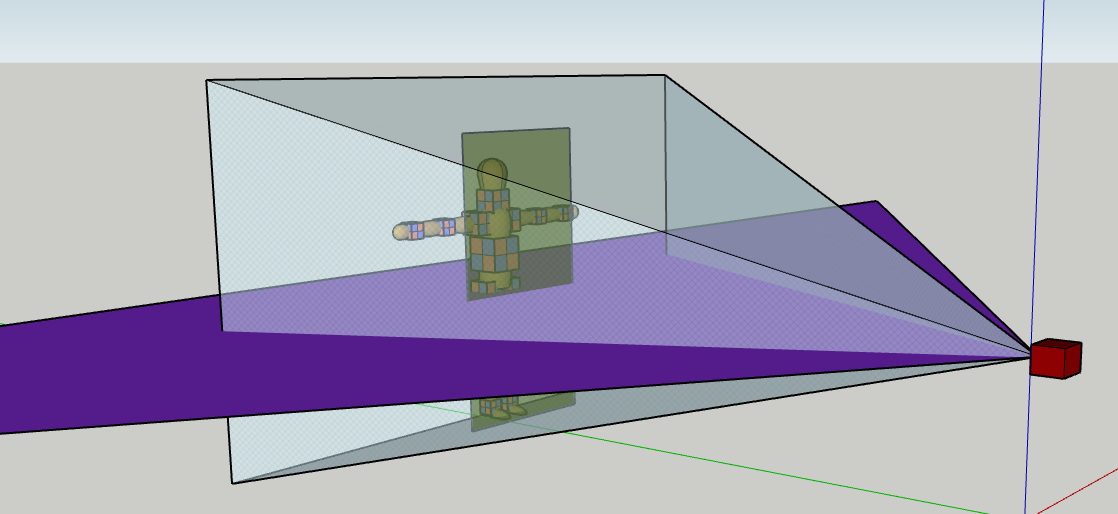
\includegraphics[scale=0.5]{different_dimensions.PNG}
				\captionof{figure}{Visualizing different dimensions measured by the M16 Lidar and Brio Webcam.}
				\label{dimensions}
			\end{figure}

		\subsection{Physical Mount Design}

		\subsection{Computer Vision}
			I started with OpenCV's pre-trained facial/pedestrian support-vector-machine (SVM) classifier.
			This SVM is a combination of several other SVMs that detect the upper body, eyes, mouths, and noses.
			The combined SVM is intended to detect faces with high accuracy.
			However, when applied to my design, I could not consistently replicate good results.
			This was due to several factors, namely the SVM used was meant to perform classification on still images where the camera's perspective is far from the subject.
			

			My design specifications envision a system that quickly tracks multiple subjects in a crowded expo scenario.
			In an expo scenario, human subjects will be moving close or away from the camera, unpredictably shifting their positions, and moving in or out of the field-of-view.
			As seen in \ref{svm}, the OpenCV SVM model does not perform to my specification.
			If the human subject were to turn their head or move too quickly, the SVM will have difficulty tracking their body.
			Additionally, the SVM performs intensive calculations on the computer's CPU, severely limiting the video output's frame-rate and resolution.
			

			\begin{figure}[H]
			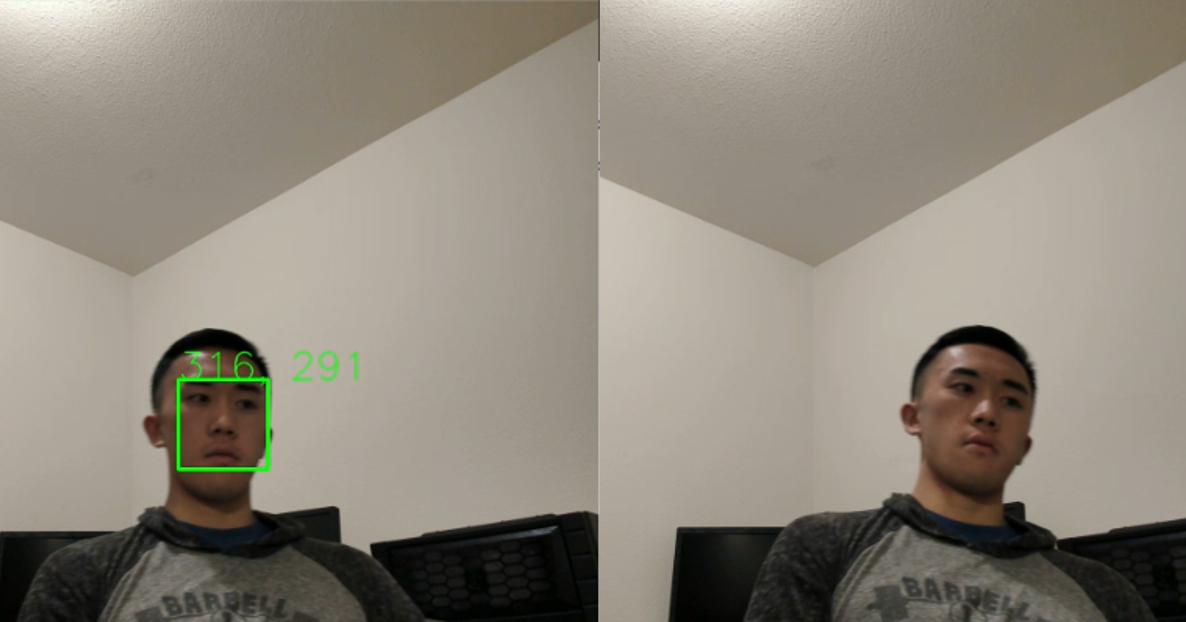
\includegraphics[scale=0.75]{svm.PNG}
			\captionof{figure}{SVM face classification (Left) fails when subject slightly turns their head (Right)}
			\label{svm}
			\end{figure}


			Recognizing the SVM's weaknesses, Tensorflow's open source object detection classifier presented a better computer-vision alternative. \cite{tensorflow}
			The Tensorflow object recognition library is better suited for this project because its library has already been trained to recognize a large dataset of objects. \cite{convolutional_object_detectors}
			These pre-trained datasets in Tensorflow's library are sourced from other machine learning datasets including the COCO dataset, Kitti dataset, and the Open Images dataset. \cite{coco} \cite{open_images} \cite{kitti}


			\begin{figure}[H]
			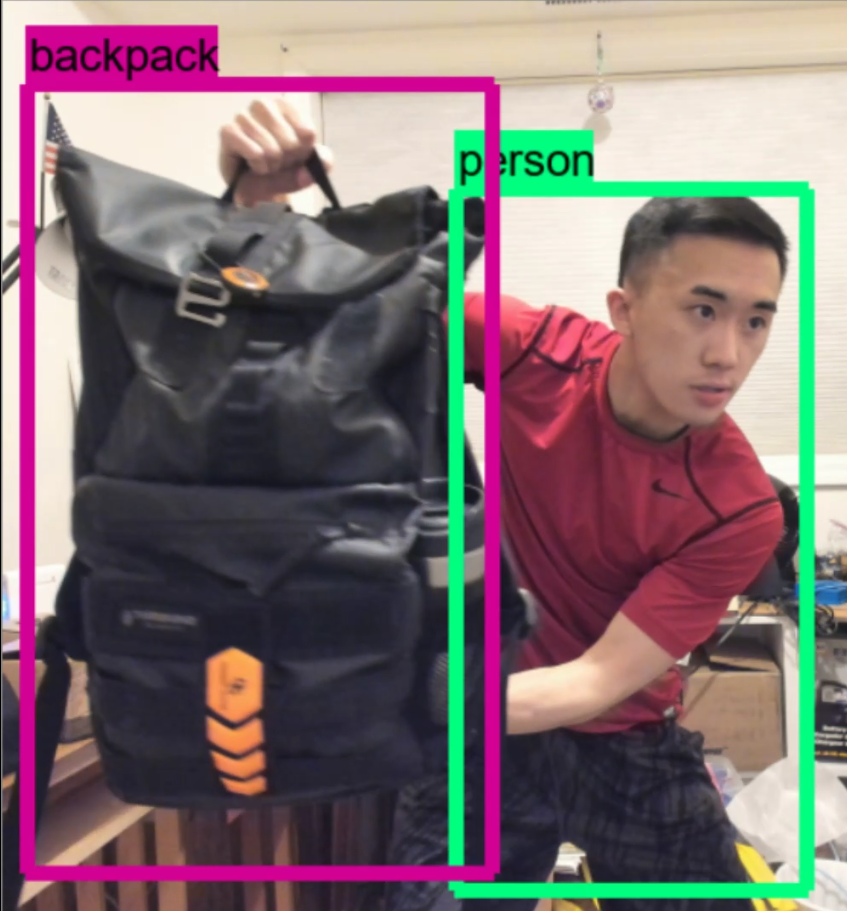
\includegraphics[scale=0.5]{tensorflow.PNG}
			\captionof{figure}{Pre-trained Tensorflow model detecting multiple subjects}
			\label{tf-detect}
			\end{figure}


			Using this pre-trained Tensorflow model, my project is now able to accurately outline and label over 90 subjects as they come into view of the webcam.
			At the end of Winter Term, the state of the code will enableselectively editing the output video frames to draw bounding boxes on subjects as they move in and out of the camera's field of view.


			Tensorflow also enables us to take advantage of NVIDIA CUDA, a driver that moves intensive calculations to the GPU.
			While this increases the list of material requisitions for demo, moving calculations to the GPU greatly improves the output video quality, frame rate, resolution, and classification speed. \cite{nvidia}
			
	\subsection{Final System Overview}


	\clearpage

	\section{Cumulative Ten-Week Term Retrospective}
		\subsection{Winter 2018}
		\begin{longtable}{|l|p{0.3\linewidth}|p{0.3\linewidth}|p{0.3\linewidth}|}\hline \textbf{Week} & \textbf{Positives} & \textbf{Deltas} & \textbf{Actions}\\\hline
		1 	&
			-
			&
				Kim says we're moving too slowly compared to previous teams
				In my opinion making a website is a far simpler task than writing code that performs analysis  and aggregates data in a system that is unproven and has never been done before

				Kim don't want us to work on filtering acceptable images even through that is what we stated we would do in our problem statement
				All problem statement drafts focused on filtering acceptable images
				None of our problem statements alluded to focusing on image analysis to interpret aerosol content
			&
				OUR TWO OPTIONS PRESENTED TO US:
				1) Kim wants us to focus on a system to interpret aerosol content in the atmosphere based on images of the horizon, EXIF data from those images, and data from wunderground
				2) (In her view) continue on this image filtering path we have started, overall this current project goal of a filter is not applicable to Aerolyzer

				I believe we have not gone astray. What I have written is relevant in either option.
				I still believe we can accomplish 1). 

				Seems like she gave up on us
				(in my opinion) we are a lower priority given our pace and low confidence in our abilities
				The code I wrote is still relevant. It will still pick out the sky which is still very necessary, it will still need to be used no matter the option we choose.

				I am the only one on Github discussing anything about the project.
				Neither Logan or Daniel have communicated to me that the direction we were going was wrong
				I don't think Kim understands the scope of the code that is necessary for a filter or why a filter is necessary
				I don't think she is reading what I'm documenting on our github or how my code is used.

			\\\hline

		2 	&
			Meeting with kevin over webex last Friday transcribed notes

			May or may not have a partner

			Usable up to 50 meters, 450 spread
			Take feed from normal webcam and overlay Leddar point cloud on video
			With minimum range and maximum range
			Device: Leddar Lydar M16
			Webcam: Logitech Brio webcam

			Most depth cameras don't work well outdoors, light sensors are overwhelmed by ambient light, overlaying point cloud on webcam video may be a way to resolve this problem

			&
			-
			&
			Research Leddar Lydar M16.
			2D Lydar unit, see if I can overlay point cloud on webcam image.
			Ideas to try:
			Research dept/distance sensing fpr 

			\\\hline

		3	&
			Talked with Lucian over email
			Unfortunately this time won't work for him, I want to keep this slot so we can at least talk, I'll leave it to him to find time to talk with you
			Gave him a quick rundown of what I understood the project to be

			He mentioned he was going to write up a problem statement and design document. 
			
			&
			Not sure exactly how to help Lucian writing the documents.
			&
			Don't need ROS (Robot operating system, don't need to use it)

			Camera depth sensor doesn’t work in sunlight, accompany with LIDAR unit

			Use realsense as point of comparison
			\\\hline

		4	&
			Borrowed Logitech brio from Kevin
			Got it working with VLC on Windows 10, set it as capture device.
			&
			Alpha stage of project = visually complete interface 
			Responsive code with placeholders for functionality
			&
			Experimenting with Brio webcam and opencv vision models.
			\\\hline

		5 	&
			Interface design?

			Suggestion: To start, draw red dot on video feed and output
			Construct internal pipeline first
			&
			Lucian and Kevin met in person for our weekly meeting, did not answer webex call so I'm not sure what they discussed.
			&
			Sent Kevin my update + screenshots and sketches of my proposed design.
			\\\hline

		6	&
			Created opencv python script to overlay green box on webcam video feed
			Successfully overlaid pixels on camera output
			Output is stuck on 4:3 resolution, going to work with it now and write code to be scalable, I want to increase ratio to 16:9 sometime, see if it's because I'm running on Linux, try with Lucian's computer later today
			&
			So the algorithmic dilemma I'm struggling with:
			We want to transfer what the lydar detects in physical 3 dimensional space into a 2D representation overlaid on a video.
			Let this white bar I've drawn here represent an offset in the y dimension (2D space in video) and z dimension (3D physical space).
			As we move our point of interest to specified distances, this angle needs to remain constant and our y/z offset needs to grow or shrink accordingly.
			This means our camera and lydar need to be stationary to define some constant angle, once that is done we can just apply some pretty simple math.
			&
			Experiment with background subtraction and opencv SVM to capture human faces.
			\\\hline

		7	&
			Lucian was talking about using some kind of equation in opencv to get distance, I think we need to get a better illustration to see how Kevin envisions us connecting the webcam feed to the data from the lydar
			&
			Sometimes I'm not sure what Lucian means.
			&
			Per my conversation with Kevin, I successfully used a trained SVM cascading front-face model to detect faces, not extremely accurate right now, thinking about using this to get face detection
			Specifically, this is needed because the Lydar will capture objects in an X-Y plane, we need the face detection to have some frame of reference in the Z direction.
			Our midterm progress report due date got pushed back, I drafted and finalized a few sections.
			Lucian wrote the other half.
			\\\hline

		8	&
			Accidently missed our poster critique session, we're going to attend the extra credit session for credit.
			&
			-
			&
			Successfuly implimented a pre-trained Tensorflow object detection model.
			This detects full or partial bodies with very high accuracy.
			After minimal tuning, the machine learning part is effectively done.
			\\\hline

		9	&
			Poster Critique session had the following suggestions: Make sure correct poster format, put figure and captions, put x-y-z scale on main image, change layout, "visually connecting" layout to have presentation flow
			Doesn’t need period at tagline
			Include contact
			Include Client
			&
			-
			&
			Made adjustments to poster design.
			\\\hline

		10	&
			Dead week, we're busy writing the Winter report.
			&
			Lucian accidentally wiped the contents and history of our documents repo.
			Fortunatly I had it cloned on my laptop so nothing was lost.
			&
			Need to discuss work schedule with Kevin and Lucian.
			\\\hline
		\end{longtable}

\end{singlespace}
\end{document}
